\documentclass[12pt,letter]{article}
\usepackage[moduleName={Pot Keys}]{KautenjaDSP}
\begin{document}
\titlePage{img/Logo}{img/Module}{img/KautenjaDSP}

% -------------------
% MARK: Overview
% -------------------

\section{Overview}

Pot Keys is an emulation of the Atari POKEY audio processing unit. The POKEY produces four pulse waveforms with a variety of bonus controls, including extended frequency ranges, retro high-pass filters, and noise generators / distortion effects. Pot Keys provides the key features of the POKEY chip, namely,
\begin{itemize}
  \item \textbf{Quad pulse wave generator:} Four pulse waves with $50\%$ pulse width and 8-bit frequency value
  \item \textbf{Low-frequency mode:} Change base clock of the chip from $64 KHz$ to $15 KHz$ for fat super-square basslines.
  \item \textbf{High-frequency mode:} Change base clock of oscillators 1 and 3 from $64 KHz$ to $1.79 MHz$ to generate high-frequency tones
  \item \textbf{High-pass filter:} High-pass filter oscillator 1 using oscillator 3 as a clock or high-pass oscillator 2 using oscillator 4 as a clock
  \item \textbf{Noise / Distortion generator:} Generate per-oscillator pseudo-random numbers at 15 different frequencies as a distortion source
  \item \textbf{4-bit Amplifier:} A 4-bit amplifier controls the output level of each oscillator with base/attenuator knobs and CV inputs
  \item \textbf{Channel Mixer:} Mix the voices together internally with hard clipping and intentional aliasing
\end{itemize}

% -------------------
% MARK: Panel Layout
% -------------------

\clearpage
\section{Panel Layout}

\begin{figure}[!htp]
\centering
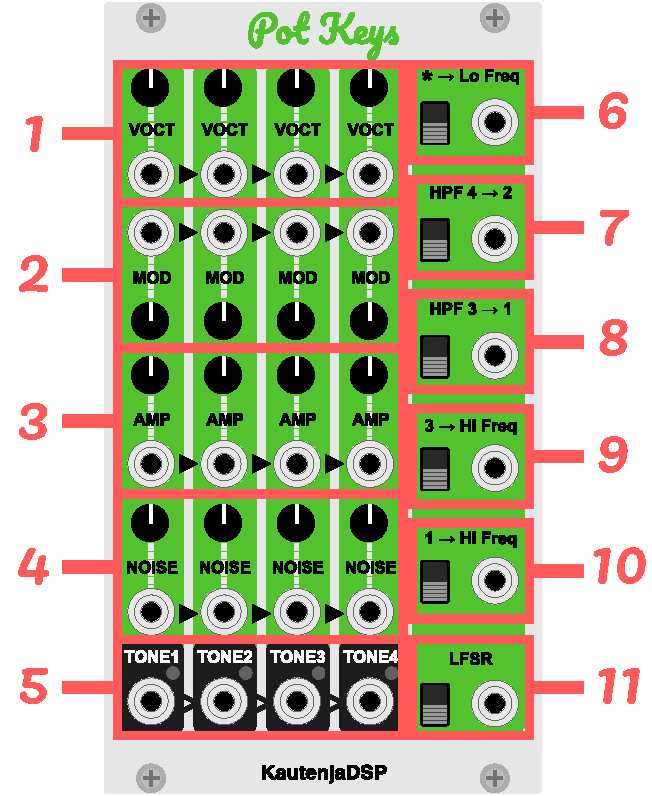
\includegraphics{img/Interface}
\end{figure}

\subsection{Frequency}

The trimpot controls the coarse frequency of the three waveform generators. Frequency is quantized to a 8-bit value for the oscillators, which is particularly noticeable in the very low / high registers. The ports provide an exponential $V$/Octave input for controlling the pitch of the tone generators. Inputs are normalled forward from Tone 1, to Tone 2, to Tone 3, to Tone 4.

\subsection{Frequency Modulation}

When nothing is patched to the frequency modulation port, the trimpot can be used to fine tune the frequency of the given waveform generator. When a signal is patched, the input port provides linear frequency modulation to the corresponding waveform generator and the trimpot can be used as an attenuverter to attenuate / polarize the incoming signal. Inputs are normalled forward from Tone 1, to Tone 2, to Tone 3, to Tone 4, and support audio rates.

\subsection{Amplifier}

When no input is connected, the trimpot controls the given waveform generator volume level with 4-bit resolution (i.e., $\in [0, 15]$). When an input is patched to the port, the trimpot acts like an attenuator that scales the CV control over the volume level. Because the amplifier has 4-bit control, the envelope of the voice will sound quantized when used with an external envelope generator. Inputs are normalled forward from Tone 1, to Tone 2, to Tone 3, to Tone 4.

\subsection{Noise}

The trimpot controls the shift register value for each oscillator's noise generator $\in [0, 7]$. Random numbers are generated by sampling the high 8 bits from the top of the 17-bit shift register. The shift register is clocked by the $1.79MHz$ clock of the chip's CPU. See Table~\ref{tab:shift-register} for a description of each shift register setting. When an input is patched to the port, the CV controls the offset from the trimpot's position. The position of the knob is offset by the CV in increments of $1V$. Inputs are normalled forward from Tone 1, to Tone 2, to Tone 3, to Tone 4.

\begin{table}[!htp]
\centering
\caption{Shift register values for the noise generators.}
\label{tab:shift-register}
\small
\begin{tabular}{|c||l|}
\hline
Mode & Description                   \\
\hline\hline
 0    & 5-bit then 17-bit polynomials \\
 1    & 5-bit poly only               \\
 2    & 5-bit then 4-bit polys        \\
 3    & 5-bit poly only               \\
 4    & 17-bit poly only              \\
 5    & no poly (pure tone)           \\
 6    & 4-bit poly only               \\
 7    & no poly (pure tone)           \\
\hline
\end{tabular}
\end{table}

\subsection{Outputs}

Each voice produces an output signal of at most $10V_{pp}$ when the amplifier is maxed out. The individual oscillators cannot be overdriven to produce clipping, distortion, or aliasing. However, outputs are normalled forward into a sum mix where hard clipping \textit{can} occur. Excess clipping will introduce an aliasing effect to the mix. Outputs in the mix are clipped \textit{before} being normalled to the next output. VU meter lights measure the output of individual channels going from off ($-\infty dB$ to $0dB$), to green ($-12dB$ to $0dB$), and lastly to red ($0dB$ to $3dB$) when clipping begins to occur.

\clearpage
\subsection{Control Register}

Each switch controls a bit in the emulated POKEY's control register described by Table~\ref{tab:audio-control}. When an input is patched to the port, CV control goes high at $2V$. The switch both flips the bit and inverts the effect of the CV input.

\begin{table}[!htp]
\centering
\caption{Descriptions of each of the bits in the Audio Control register.}
\label{tab:audio-control}
\small
\begin{tabular}{|l|l||l|l|l|}
\hline
 Bit & Name              & Description                                            & 0        & 1          \\
\hline\hline
 1   & \texttt{LOW FREQ} & Choice of frequency divider rate for all oscillators      & $64 kHz$ & $15 kHz$   \\
 2   & \texttt{HP 4>2}   & High-pass filter for Ch. 2 rated by frequency of Ch. 4 & Off      & On         \\
 3   & \texttt{HP 3>1}   & High-pass filter for Ch. 1 rated by frequency of Ch. 3 & Off      & On         \\
 % 4   & \texttt{16=4+3}   & Combine Ch. 4 \& Ch. 3 to achieve 16-bit frequency     & Off      & On         \\
 % 5   & \texttt{16=2+1}   & Combine Ch. 2 \& Ch. 1 to achieve 16-bit frequency     & Off      & On         \\
 6   & \texttt{AUD3HI}   & Channel 3 clock divider frequency                      & $64 kHz$ & $1.79 MHz$ \\
 7   & \texttt{AUD1HI}   & Channel 1 clock divider frequency                      & $64 kHz$ & $1.79 MHz$ \\
 8   & \texttt{LFSR}     & Noise / distortion shift register                      & 17-bit   & 9-bit      \\
\hline
\end{tabular}
\end{table}

% -------------------
% MARK: Data Sheet
% -------------------

\clearpage
\section{Data Sheet}

\begin{table}[!htp]
\begin{tabular}{|l|l|}
\hline
Type             & Oscillator               \\
\hline
Size             & 14 HP Eurorack           \\
\hline
Depth            & NA                       \\
\hline
Power            & NA                       \\ % 2 x 5 Eurorack
\hline
$+12V$ draw (mA) & 0 mA                     \\
\hline
$-12V$ draw (mA) & 0 mA                     \\
\hline
$+5V$ draw (mA)  & 0 mA                     \\
\hline
Sample Rate      & Programmable             \\
\hline
Bit Depth        & 16-bit                   \\
\hline
\end{tabular}
\end{table}

% -------------------
% MARK: References
% -------------------

\clearpage
\renewcommand\refname{References}
\nocite{*}
\bibliographystyle{apalike}
\bibliography{references}

\end{document}
